% !TEX encoding = UTF-8
% !TEX TS-program = pdflatex
% !TEX root = ../Tesi.tex
% !TEX spellcheck = it-IT

%************************************************
\chapter{Appunti sul marmo}
\label{cap:appunti}
%************************************************

\section{Note di programma}

Qui, l’incedere di una risonanza è legata ad un corpo/luogo, lentamente mutabile:
uno spazio che è memoria di superficie. Abitare questo ascolto è stato il primo
passo della scrittura, il formalizzarsi e il perdersi di una molteplice voce,
abitante abitato da \emph{per sempre}.

Partenza (come dipartita), della stessa scrittura strumentale tradizionale. 
Lo studio dello spazio di \emph{San Luca} ha instaurato diverse relazioni che
congiungono i diversi strati di elaborazione, dalla macro alla micro-struttura.

\section{Coscienza di scrittura}

L'immemorialità dell'evento scandisce sia il gesto formale che la struttura,
organizzando i contributi qualitativi del suono e la loro distribuzione
temporale e spaziale. Immemorialità dello stesso suono come strumento trasformato
e non riconducibile a:

\begin{description}
	\item[ Altezza temperata ] È volutamente ricercato nello strumento la sua
	oscillazione  attorno a dei poli frequenziali (descritti successivamente),
	cercando la massima \emph{instabilità-controllata}. Giochi di oscillazione che
	intercorrono tra l’evidente parametro multifonico e la sua de-costruzione
	timbrica. Lo stesso vale per i battimenti, altri importanti operatori di
	trasformazione.
	\item[ Modalità di emissione eterogenea ] Gradazioni controllate di soffio e
	suono, oltre che intonazione di aberrazioni prodotte tramite saliva e
	spostamento dell'imboccatura.     
\end{description}

\begin{figure}[h]
\centering
{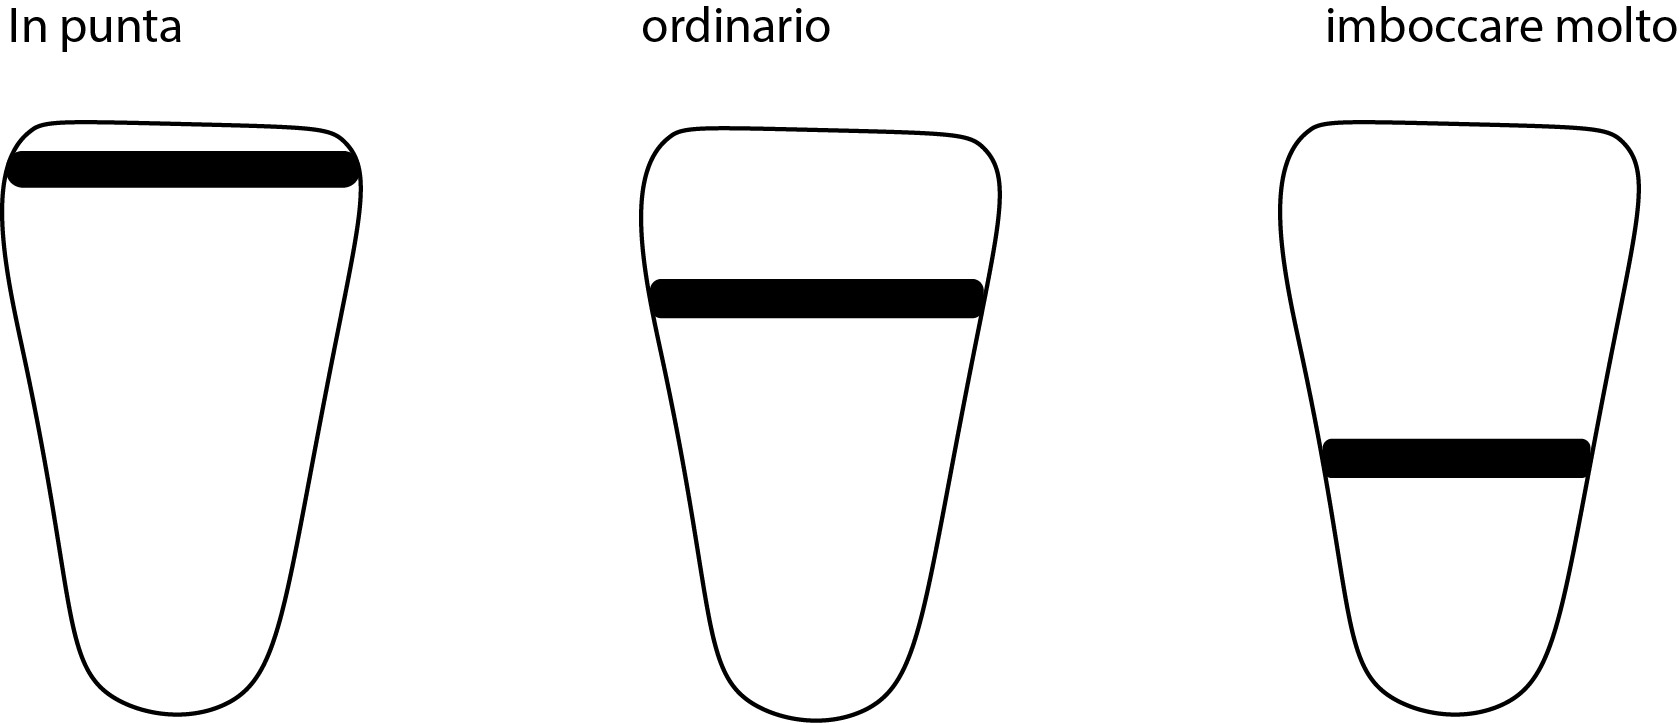
\includegraphics[width=.65\columnwidth]{sax_boc.jpg}}
\caption[Schemi imboccatura]{Schemi imboccatura}
\label{fig:imboccatura}
\end{figure}

\section{Perché il sassofono?}

Le caratteristiche cercate in questo strumento si basano sulla possibilità
di insistere su determinati fattori; il corpo/bocca dello strumentista,
le modifiche della colonna armonica, i suoi armonici sovracuti, doppiati
e triplicati nel medesimo tempo/istante.
Il sassofono soprano rende possibile la continua modulazione tra multifonici:
una “corrente continua”,  dove il movimento lento (pensato assieme all'impronta
elettronica del luogo) permette lo stazionamento di determinate parziali
e il passaggio fluido tra differenti bicordi. È stato fondamentale lo studio
dei parziali multifonici, il loro isolamento monodico e la possibilità di
“entrare” ed “uscire” dalla posizione di generazione multifonica.

Possiamo dividere le qualità di queste parziali in famiglie:

\begin{description}
	\item[ --- ] parziali \emph{treshold tones}
	\item[ $ \sim $]  \emph{shadow sound}, suoni che non possono essere i solati.
	È stato posto l’accento sulle possibili aberrazioni che si pongono su ottave differenti
	rispetto al suono cardine, rendendo il contenuto spettrale più instabile e ricco.
	\item [ $ \supset\supset\supset $] \emph{instabile}. Alcune regioni frequenziali di multifonici presentano una
	difficile risposta. Battimenti o parziali sovracuti avranno una risposta non lineare.
	Si deve tendere a cercare una sorta di \emph{modulazione di ampiezza}.
	Cercare il suono\footnote{i simboli sono presi dal trattato di Weiss e Netti}.
\end{description}

Conseguenziale a questo tipo di scrittura è il rapporto e la pratica con lo strumentista.
Le tecniche estese di partenza vengono dagli studi di Weiss e Netti, ma il percorso di
elaborazione, di nuova scoperta di emissione e modulazione di timbro e altezze è
stato condotto assieme al sassofonista Danilo Perticaro.

\clearpage

~

\clearpage

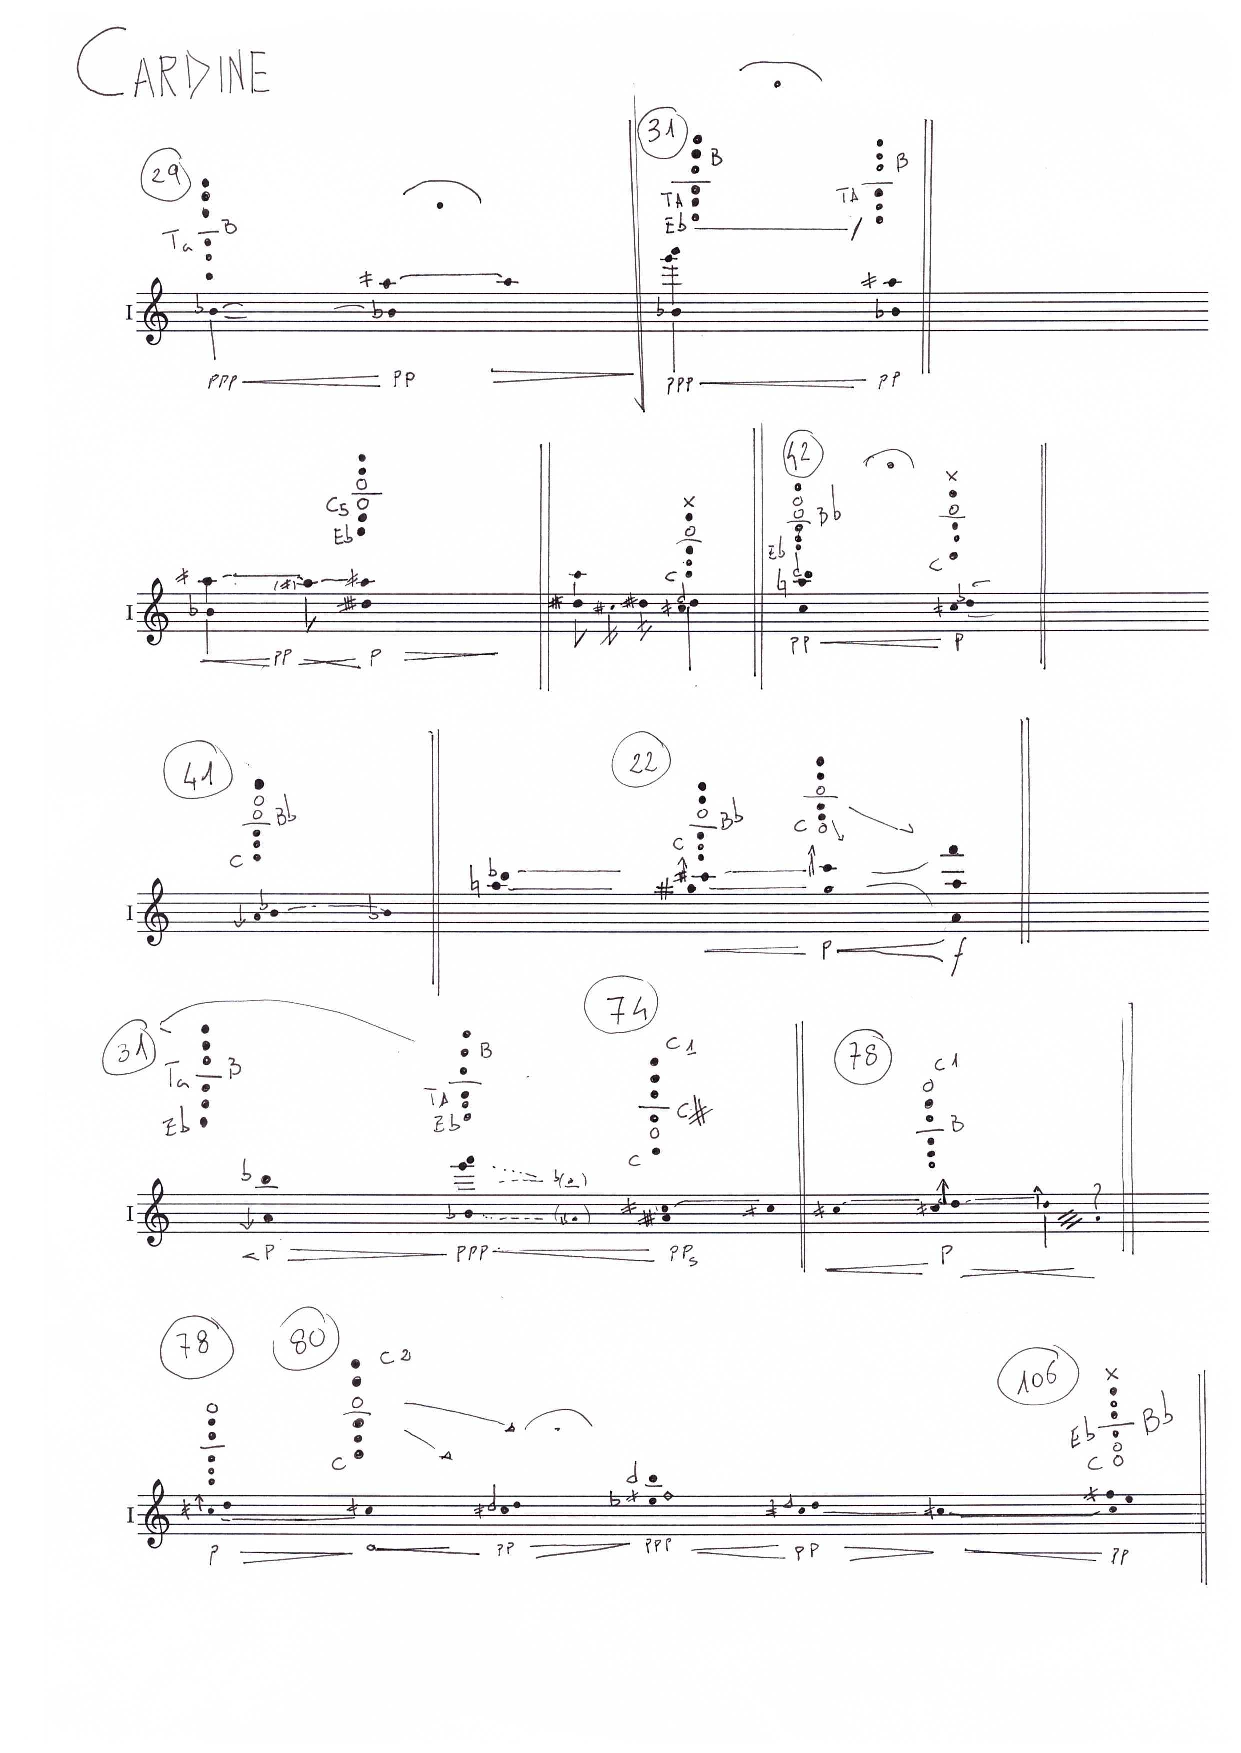
\includepdf[scale=0.9]{Suoni-Cardine-1.pdf}

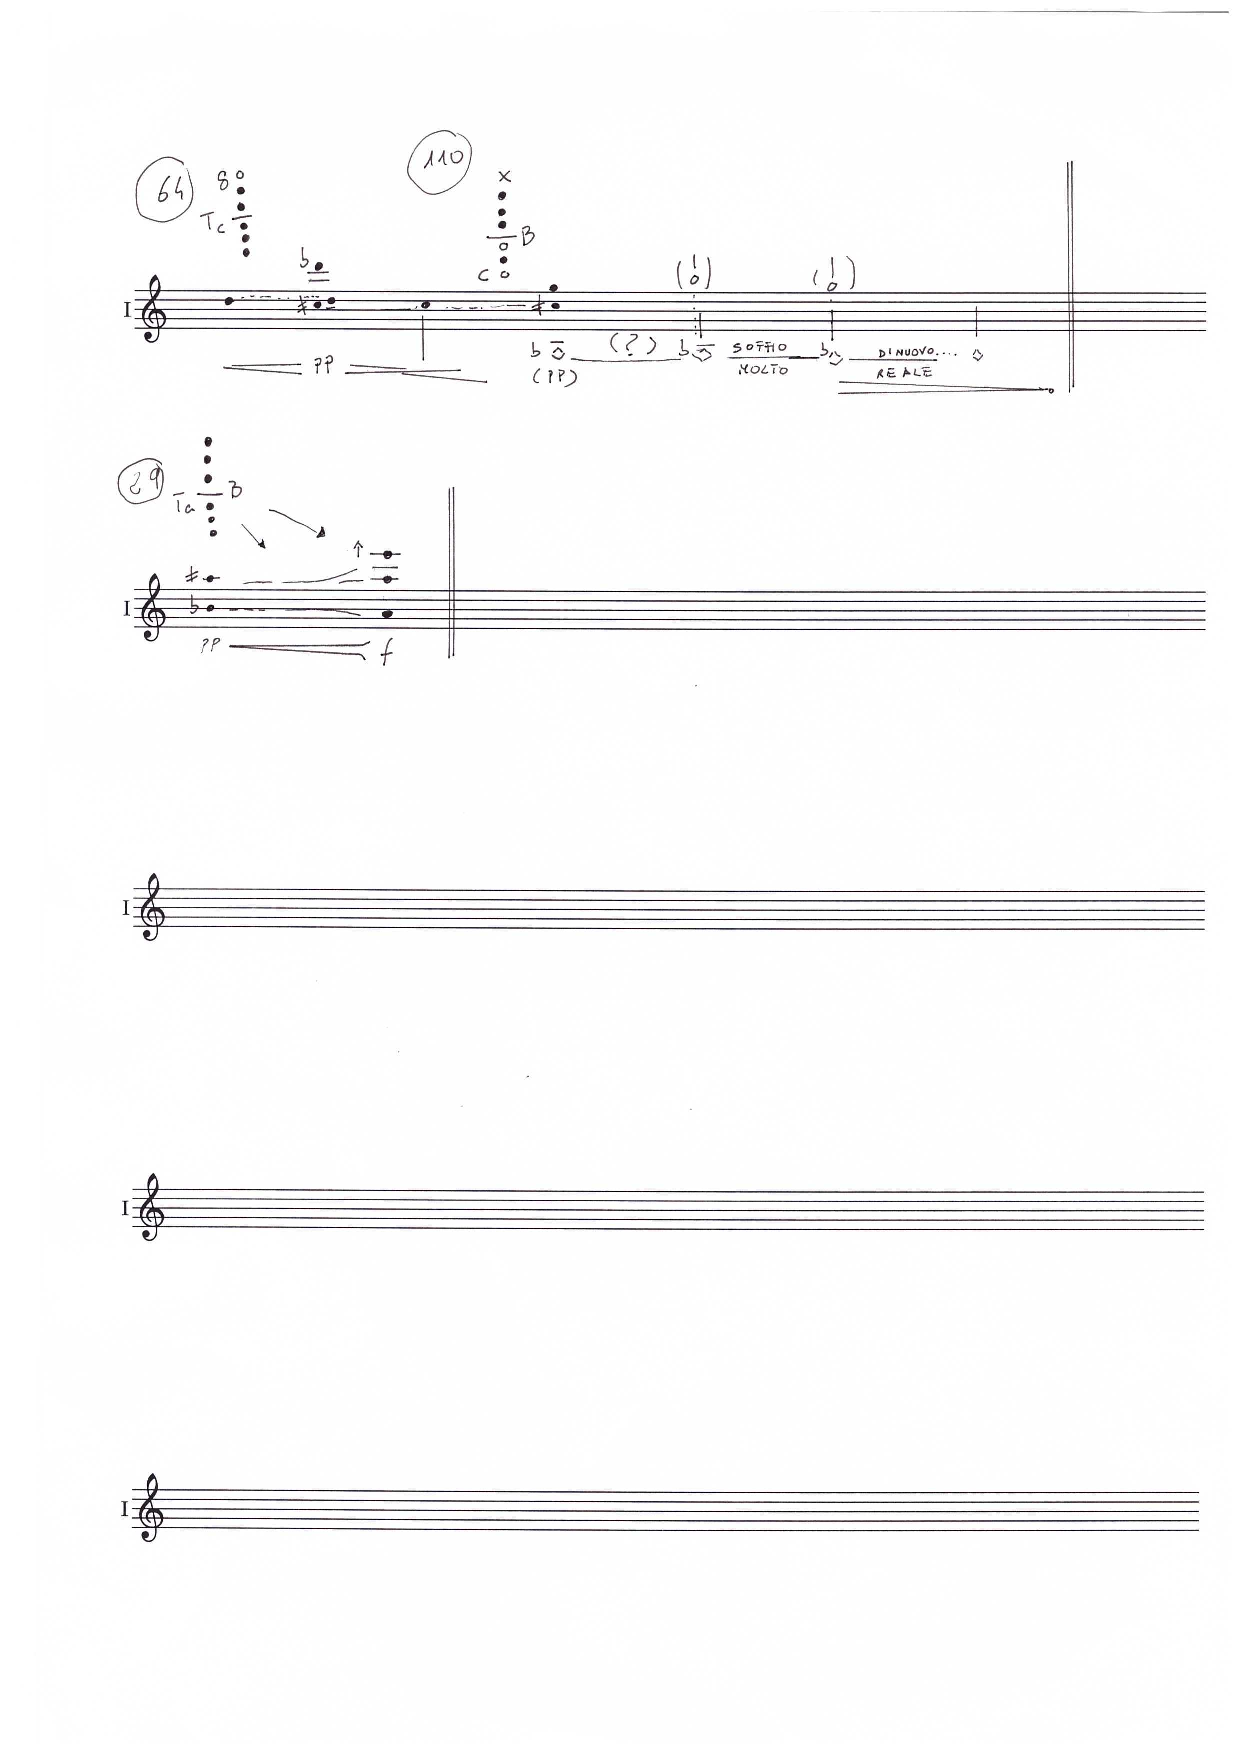
\includepdf[scale=0.9]{Suoni-Cardine-2.pdf}

Qualità sonore e trasformazione suoni cardine del brano\footnote{Alcune delle transizioni
e multifonici non si trovano nel brano. Gli schemi preparatori riportano anche lavoro a
monte rispetto allo studio con lo strumentista.  Provandoli successivamente ci siamo
resi conti di incongruenze legate alla difficolta di diteggiatura o differente
legatura di emissione (dinamiche eccessivamente differenti portavano ad non legare le posizioni)}
Ogni diteggiatura nel suo legarsi presenta un effetto di modifica non solo
frequenziale ma dello spettro stesso delle parziali.

Ogni diteggiatura nel suo legarsi presenta un effetto di modifica non solo frequenziale ma
dello spettro stesso delle parziali. La logica d'uso di queste tecniche si pone
lontana dagli schematismi di \emph{effetto} che ruotano attorno all'articolazione di note. 

\vfill

\begin{figure}[h]
\centering
{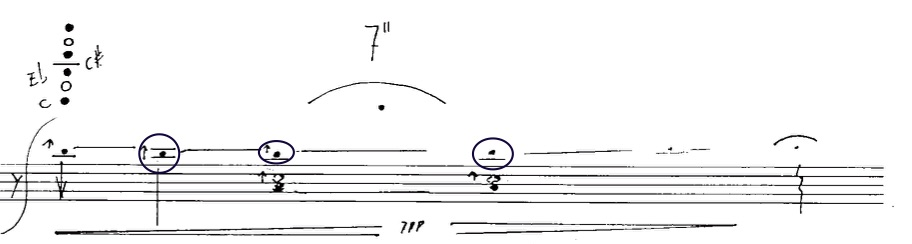
\includegraphics[width=.75\columnwidth]{parziali-sovracuti.jpg}}
\caption[Assottigliamento verso i suoni sovracuti]{Assottigliamento verso i suoni sovracuti del sassofono (materiale povero spettralmente)}
\label{fig:assottiglimento}
\end{figure}
 
\vfill

\begin{figure}[h]
\centering
{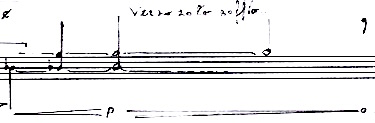
\includegraphics[width=.65\columnwidth]{filec.jpg}}
\caption[Emissione - soffio - battimento]{Emissione - soffio - battimento}
\label{fig:soffio}
\end{figure}

\vfill
 
\begin{figure}[h]
\centering
{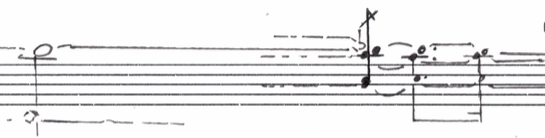
\includegraphics[width=.55\columnwidth]{fileA.png}}
\caption[Passaggio microtonale]{fondamentale-parziale accrescimento-svuotamento}
\label{fig:microtoni}
\end{figure}

\section{Environment}

La logica spaziale proposta con la risposta all'impulso e la riproduzione tramite sistema
tetraedrico, ha portato a concepire un uso delle fonti sonore che gravitano interne e
all’esterno dell'ambiente della chiesa di San Luca.

La registrazione e la riproduzione tramite sistema \emph{A-format} permetteva di delineare una
cartografia tridimensionale degli eventi: tramite un'azione musicale preparata sono stati
controllati e scanditi i materiali suonati all'interno della chiesa: preparata in quanto
si vuole nascondere il più possibile l’evento acustico dalla percezione familiare, dal
suo effettivo sguardo \emph{concreto}.

La logica di registrazione segue il quadrante interno alla chiesa utilizzato per gli impulsi.

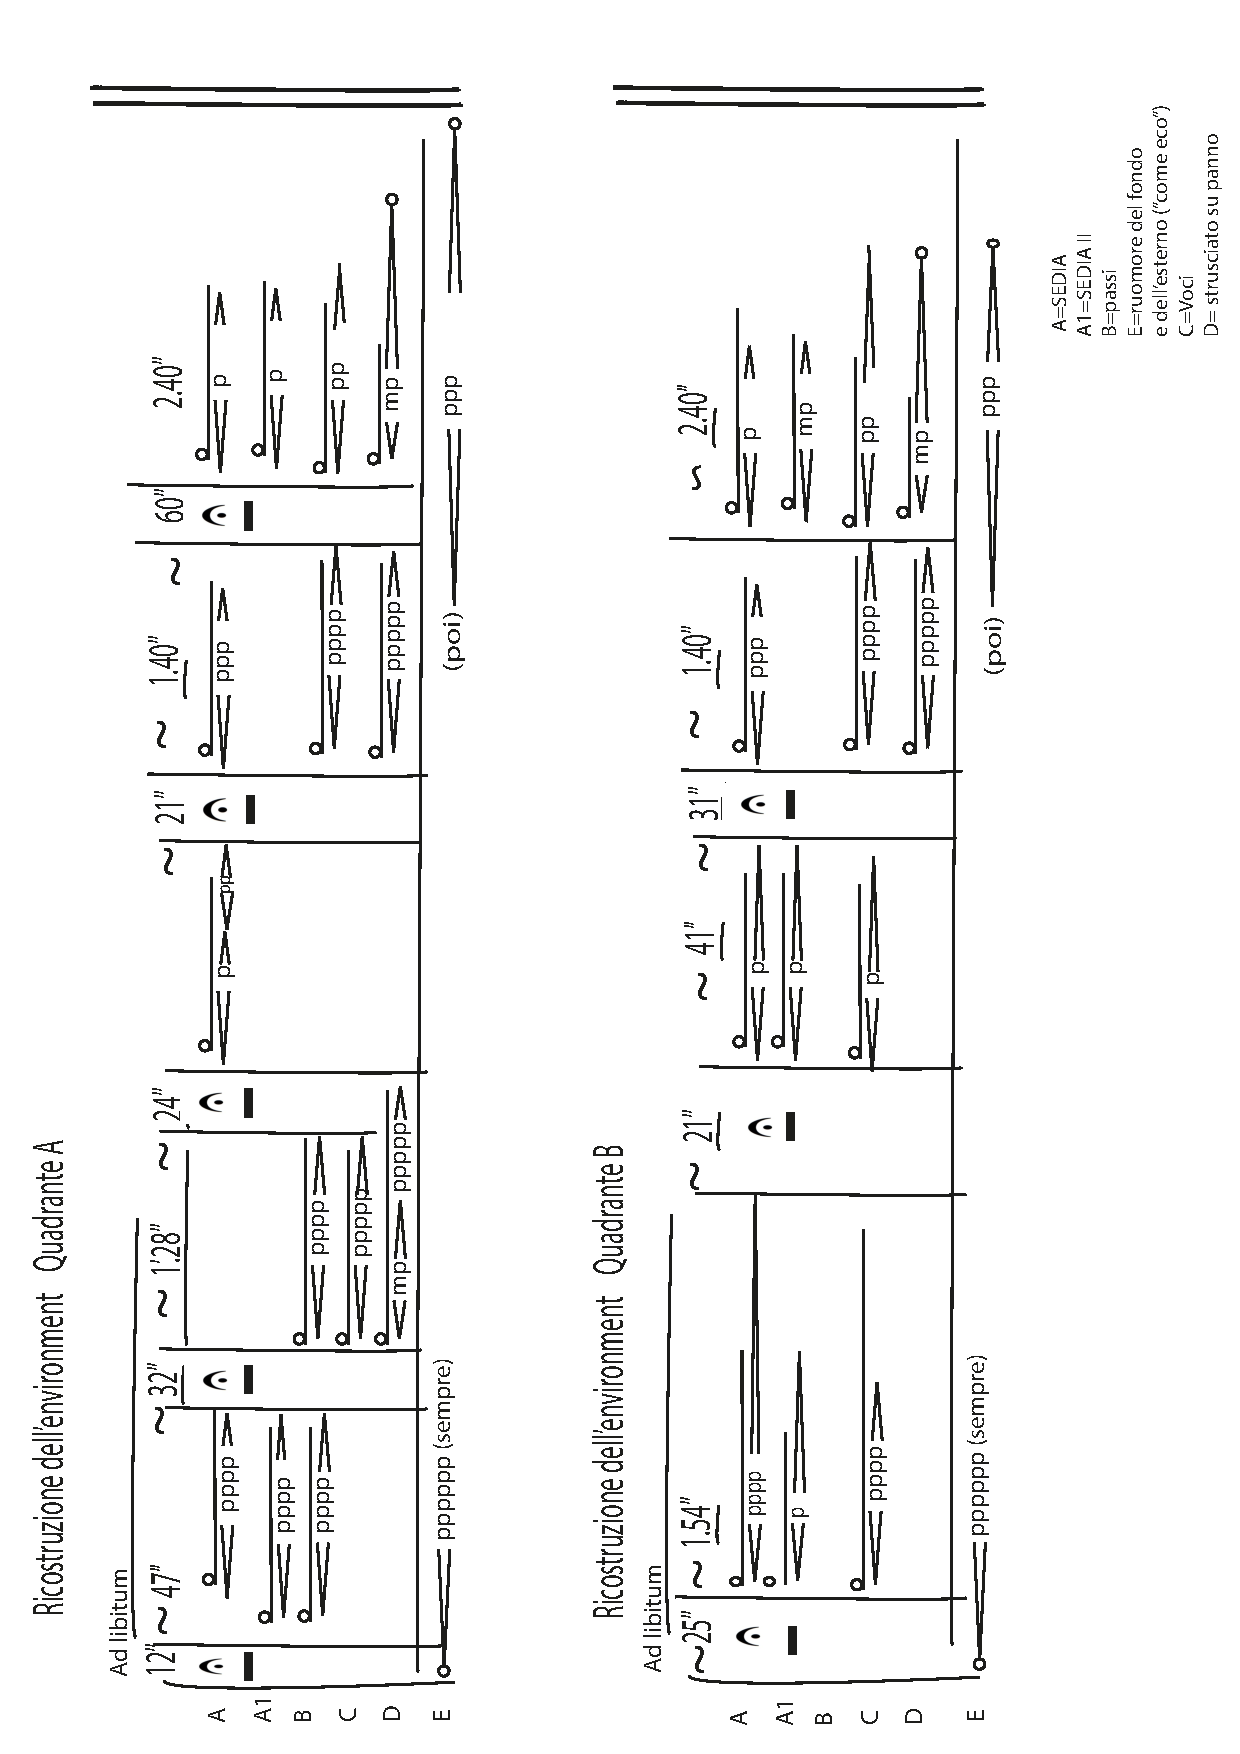
\includepdf[scale=0.9]{Tape.pdf}

\begin{figure}[h]
\centering
{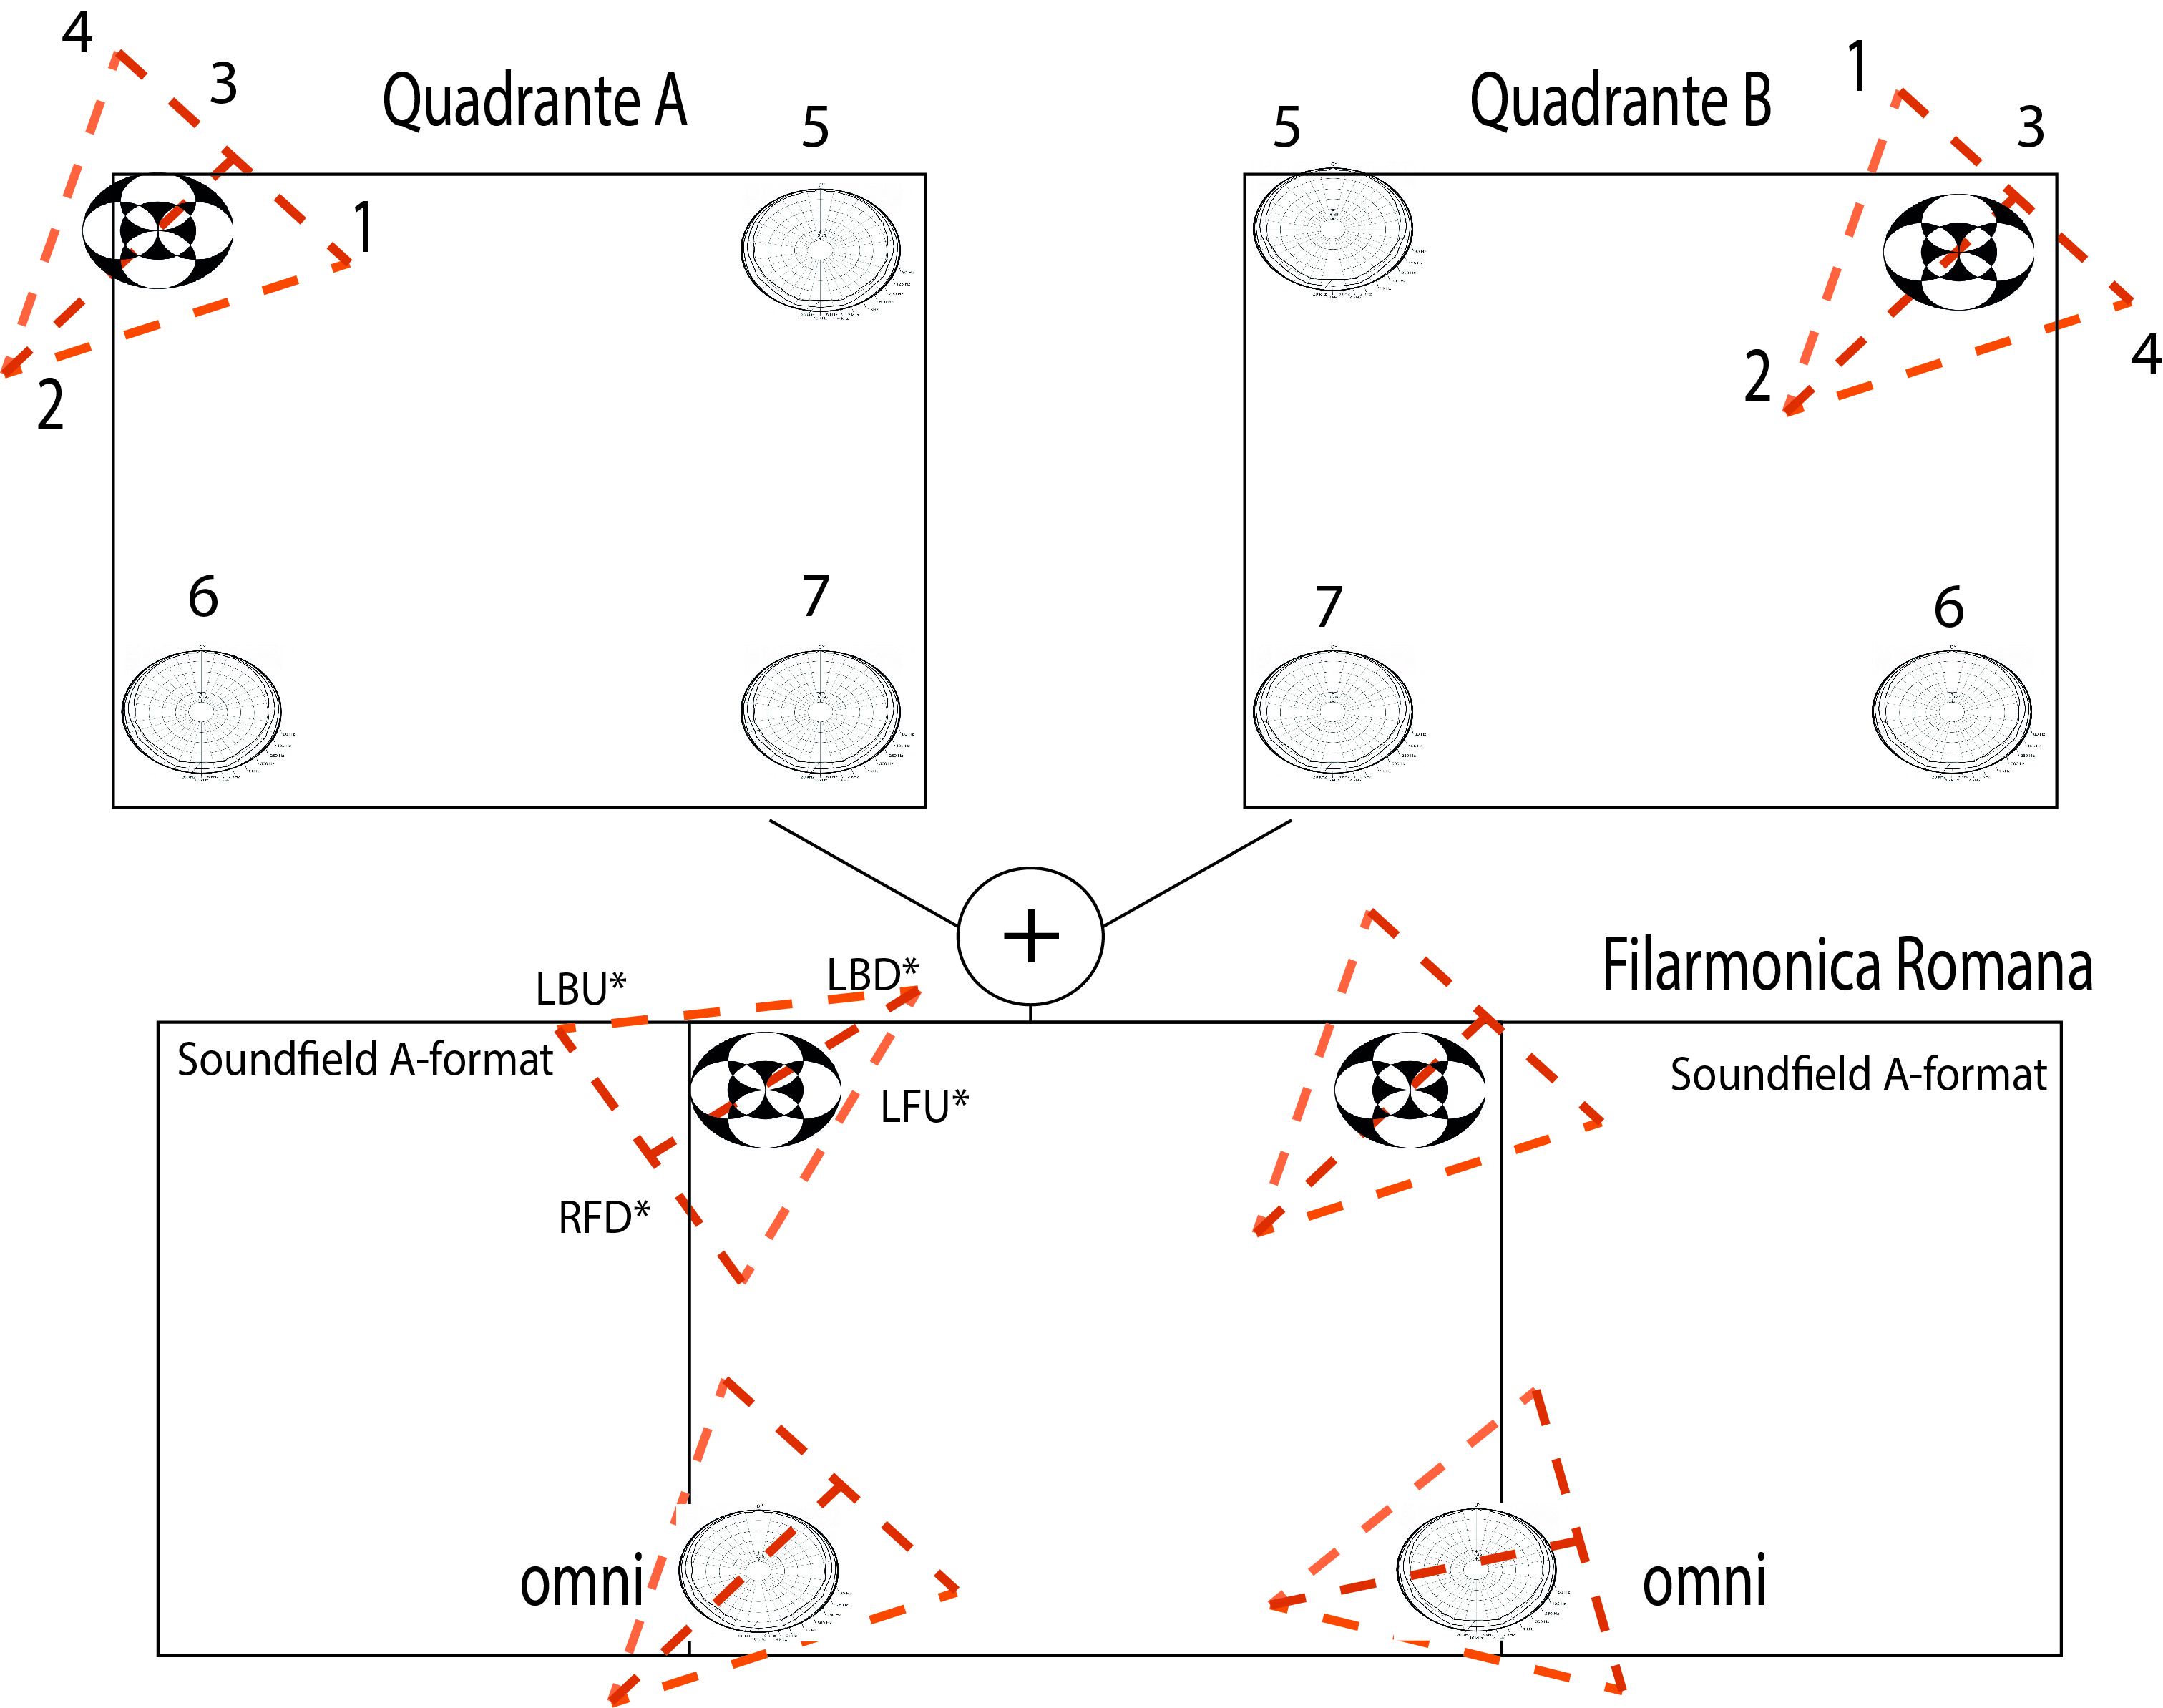
\includegraphics[width=.95\columnwidth]{quadranteaeb.jpg}}
\caption[Passaggio microtonale]{fondamentale-parziale accrescimento-svuotamento}
\label{fig:microtoni}
\end{figure}

\subsection{struttura del nastro}

La preparazione del nastro richiede tre esecutori                                                            
la durata del nastro è di circa 10 minuti.
è da considerare ad libitum. Sarà chiuso il processo da parte del regista del suono.
L'incontro con la parte strumentale è fortemente aleatoria. Environment attorno all’ascoltatore,
attorno allo strumentista, con banda medio-grave. È possibile riscrivere il nastro
partendo dai materiali e dallo schema relativo alle dinamiche generale. Il tutto deve
essere tra \ppp\ppp ~ e \pp .

\bigskip

MATERIALI:

\begin{enumerate}
	\item [A] ambiente esterno alla chiesa \newline (controllare adeguatamente il livello d'ingresso del soundfield)
	\item [B] banchi da chiesa (scricchiolio)
	\item [C] sedie
	\item [D] passi
	\item [E] voci
\end{enumerate}

La scelta di preparare  dal vivo il materiale  concreto e non elaborarlo successivamente
è dato dal fatto che i 4 tape registrati dal soundfield potevano andare incontro a
sfasamenti togliendo la componente tridimensionale. Solo tagli e riposizionamenti
del nastro, entrate ed uscite delle tracce.

Sono state registrate due azioni con una configurazione dei microfoni diversa,
per poi essere integrati nell'esecuzione:

\begin{center}
quadrante A + quadrante B
\end{center} 

Come si vede dallo schema la tridimensionalità del nastro è prevista solo per i due
\emph{S.T.ONE} frontali, paralleli alla posizione dello strumentista. Sugli altri due
\emph{S.T.ONE} è prevista diffusione monofonica, omnidirezionale.

\begin{figure}[h]
\centering
{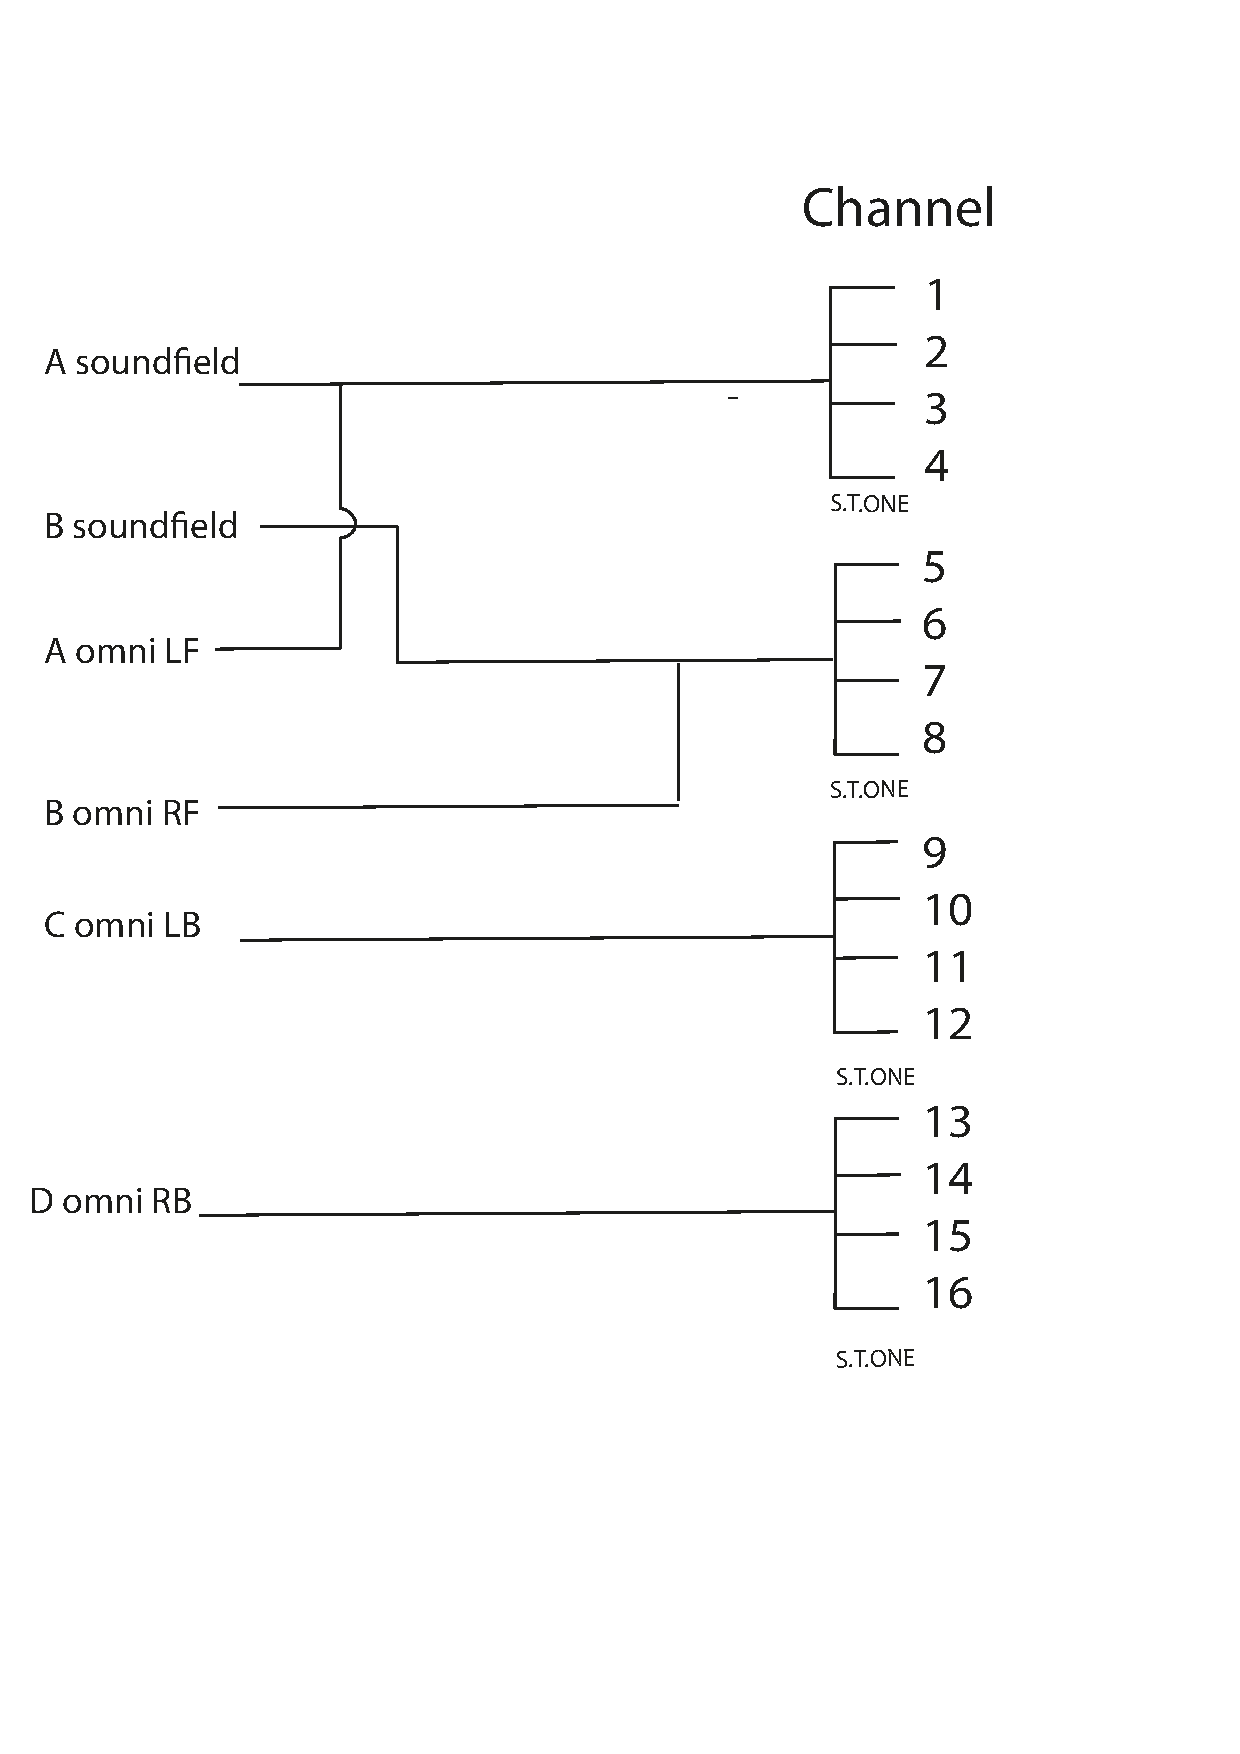
\includegraphics[width=.9\columnwidth]{MICROFONI.pdf}}
\caption[Passaggio microtonale]{fondamentale-parziale accrescimento-svuotamento}
\label{fig:microtoni}
\end{figure}

\section{La discesa come struttura}

Il tragitto costruito tramite il sassofono soprano è direttamente intrecciato alle sue
possibilità più remote, ad uno studio acustico che insiste sulla transizione di bicordi.
Un passaggio da un certo grado intervallare a l’altro, in una continua trasformazione,
pronta ad dilatarsi in un tempo immobile. Questo gioco, del perdersi e riprendersi
variando nei registri e nelle  qualità vibrazionali, mette in relazione luoghi
acustici eterogenei dalla ricca complessità timbrica.
Luogo,scrittura, concepito nelle possibilità che ogni passo, gradazione nata dal
primo bicordo di sesta minore, poteva mettere in gioco: l’individuazione del successivo
istante e cambio di frequenze è circoscritto alle posizioni di chiave appena precedute.
Il successivo bicordo è in molti dei casi costituito da una delle parziali che fa da
ponte tra un intervallo e l altro.
Questa successione di eventi (rizoma tra due voci poste ora in accordo poi battimento)
è il fondamento della struttura, dell’alveare polifonico e microtonale.
Le tecniche estese consentono di sfruttare parziali inarmoniche, tipiche di questo
strumento, organizzando dei poli microtonali.

Prendo in esempio l’evento generante che gravita attorno alla frequenza del si{\large$\flat$}5.

Il successivo movimento tiene conto di questo polo alterando l’intervallo a favore
di un spostamento quartitonale, per poi riassumere nei succesivi movimenti l’aspetto originario:

È comunque da tenere conto che i microtoni non sono pensati su una scala temperata ma
in riferimento alla serie delle parziali del sassofono soprano. 

Possiamo prendere come intervalli polari-circostanziali:

\begin{center}
sesta minore-quinta aumentata
\end{center} 

\begin{center}
seconda minore-battimento 
\end{center} 

La qualità del battimento è fondamentale e questa trasformazione entro la seconda minore.

Esso è “interruttore” per lo spostamento del polo.

Il progetto di queste polarità frequenziali è andato di pari passo con quella di
relazioni alla costruzione di qualità descritte in precedenza.

\subsection{Klangqualitätemelodie}

-variazioni delle qualità attorno ai poli. tipo di variazione

-operatori di instabilità

-variazione informale

 poietica : discorso con danilo

Due Luoghi macroformali


la divisione della struttura è data dalla predominanza di determinati poli che scandiscono  le due luoghi macroformali.




\part*{appunti sul marmo - partitura}



